\documentclass{article}

\usepackage[dutch]{babel}
\usepackage[margin=3cm]{geometry}
\usepackage{graphicx}

\graphicspath{
    {img/}
} 

\newcommand{\bold}[1]{\textbf{#1}}
 
\begin{document}

\begin{titlepage}
    \author{Tuur Vanhoutte}
    \title{Sensors \& Interfacing}
\end{titlepage}

\pagenumbering{gobble}
\maketitle
\newpage
\tableofcontents
\newpage

\pagenumbering{arabic}

\section {Communicatie}
\subsection{Datacommunicatie in IoT}
3 lagen:
\begin{enumerate}
    \item Application Layer
    \item Fog layer
    \item IoT Device Layer
\end{enumerate}

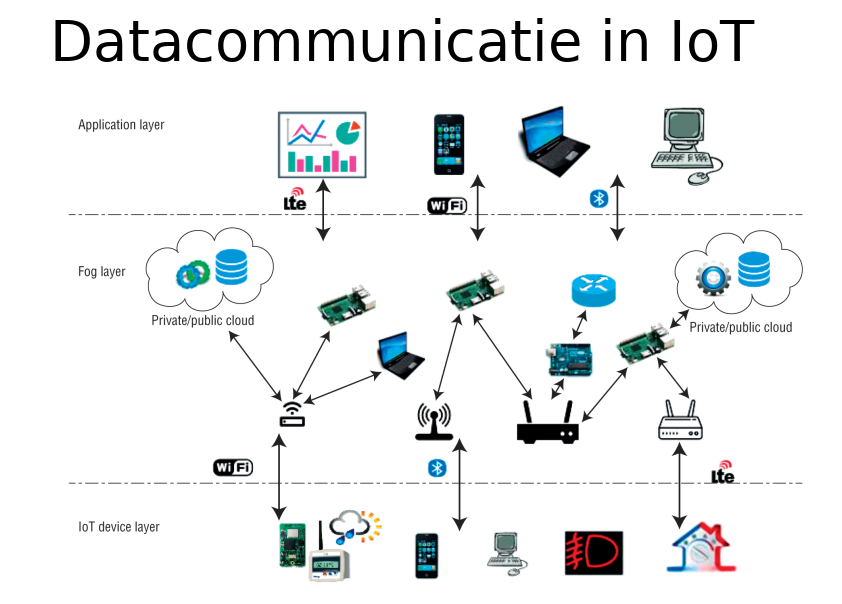
\includegraphics[width=0.95\textwidth]{Screenshot_20200210_120010.png}

\subsection{Data}
\begin{itemize}
    \item "Pre-informatie"
    \item Gegevens waaruit informatie kan worden gewonnen
    \item Stelt een bepaalde toestand voor
\end{itemize}

\subsection{Communicatie}
Overbrengen van informatie tussen deelnemers
\begin{itemize}
    \item Boodschap
    \item Signaal
    \item Medium
\end{itemize}

\subsubsection{Communicatieafspraken}
\begin{itemize}
    \item Coderen van informatie (encoding)
    \item Voorbeeld:
        \item morse-code
        \item Ascii-codering
        \begin{itemize}
            \item Codering voor alle gebruikte symbolen in symbolen
            \item Codering in 7 of 8 bit
            \item 1 byte = 1 teken
        \end{itemize}
        \item \dots
\end{itemize}
  
\subsubsection{Encoding/Decoding}
\begin{enumerate}
    \item Codifying
    \item Sending the message
    \item Decodifying
\end{enumerate}

\subsubsection{Signalen}
\begin{itemize}
    \item Licht
    \item Geluid
    \item Elektriciteit
    \item \dots
\end{itemize}

\subsubsection{Communicatiemedia}
\begin{itemize}
    \item Twisted-Pair cable
    \item Coaxial cable
    \item Fiber-Optic cable
\end{itemize}

\subsubsection{Voorbeelden}
\begin{itemize}
    \item Welke codering?
    \item Wat is het signaal?
    \item Wat is het medium?
\end{itemize}

\subsubsection{Eigenschappen van media}
\begin{itemize}
    \item Vatbaarheid voor interferentie
    \item Overbrugbare afstand
    \item Praktisch
    \item Kostprijs
\end{itemize}

\subsubsection{Afspraken}
\begin{itemize}
    \item Protocol
    \item Standaarden
    \item IEEE
    \item EIA (NEDA/ECA)ECIA
\end{itemize}

\subsubsection{Standaardiseren van \dots}
\begin{itemize}
    \item Type media en zijn specificaties
    \item Het gebruikte signaal en zijn toleranties
    \item De elektrische interferentie
    \item De gebruikte codering
    \item Foutcorrectiecodes
    \item Protocol
    \item De gebruikte connector
    \item \dots
\end{itemize}

\section{Analoog vs digitaal}
\begin{itemize}
    \item \bold{Digitaal}: Discrete waarden
    \item \bold{Analoog}: Continue waarden
\end{itemize}
\subsection{Toestanden}
\subsubsection{Bepaalde toestand}
\begin{itemize}
    \item Temperatuur
    \item Licht aan/uit
    \item Afstand
    \item Tijd
    \item \dots
\end{itemize}

\subsubsection{Digitale toestanden}
\begin{itemize}
    \item Licht aan/uit
    \item Deur open/dicht
    \item Keuze van versnelling N - 1 - 2 - 3 - 4 - 5 - R
    \item Ruitenwisser interval uit - interval - traag - snel
    \item \dots
\end{itemize}

\subsubsection{Analoge toestanden}
\begin{itemize}
    \item Tijd (!)
    \item Temperatuur
    \item Luchtdruk
    \item Luchtvochtigheid
    \item Afstand
    \item \dots
\end{itemize}


\subsection{Signalen}
\begin{itemize}
    \item Analoog signaal
    \item Digitaal signaal
\end{itemize}

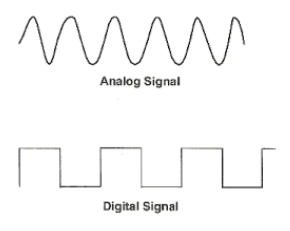
\includegraphics[width=0.4\textwidth]{Screenshot_20200217_115642.png}

\section{Analoge signalen}

\subsubsection{Transducer}
Omzetten van een analoog signaal naar een ander analoog signaal.\\
\bold{Voorbeeld}: elektrisch signaal omzetten naar een geluidsignaal via een luidspreker (=de transducer)

\subsubsection{Sensoren en Actuatoren}
\begin{itemize}
    \item Sensor $\Rightarrow$ meten van een fysieke eigenschap
    \item Actuator $\Rightarrow$ be"invloeden van een fysieke parameter $\Rightarrow$ transducers 
\end{itemize}

\subsection{Analoge communicatie}
Sinusgolf als meest elementaire signaal

\subsubsection{Eigenschappen}
\begin{itemize}
    \item DC vs AC
    \item Polariteit blijft gelijk bij (pulserende) DC
    \item Polariteit verandert bij AC
\end{itemize}

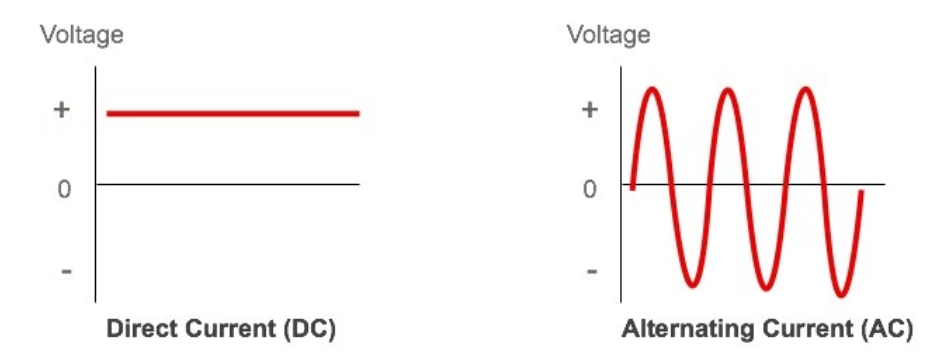
\includegraphics[width=0.5\textwidth]{Screenshot_20200217_121011.png}

\subsubsection{Wisselspanning - Eigenschappen}
\begin{itemize}
    \item RMS = Root Mean Square (= kwadratisch gemiddelde) = effectieve waarde (in geval van sinus)
    \begin{enumerate}
        \item Som van alle kwadraten (= square)
        \item Die som delen door het aantal waardes (= mean)
        \item Neem de vierkantswortel van dat getal
    \end{enumerate}
    \begin{itemize}
        \item Wordt vaak gebruikt in de elektriciteit om het gemiddelde vermogen te vinden
    \end{itemize}
    \item Frequentie
    \item Periode
    \item Amplitude
    \item Peak of top-to-top waarde
\end{itemize}
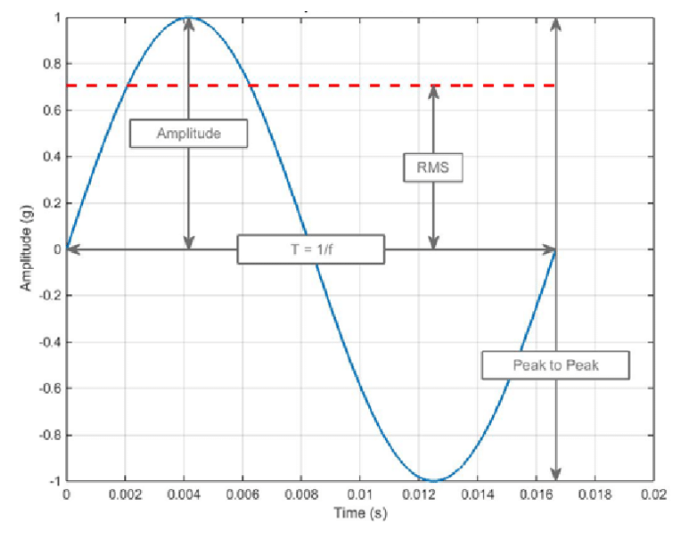
\includegraphics[width=0.7\textwidth]{Screenshot_20200217_121136.png}

\subsubsection{Periodieke signalen}
\begin{itemize}
    \item 1 herhaling = 1 periode
    \item Periode (T) = tijdsduur (in s)
    \item Frequentie (f) = aantal periodes per seconde (in Hz)
    \item $F = \frac1T$ en $T = \frac1F$
\end{itemize}

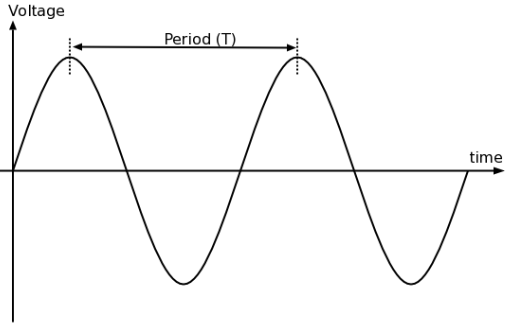
\includegraphics[width=0.7\textwidth]{Screenshot_20200217_122002.png}

\subsubsection{Tijdsdomein en frequentiedomein}
\begin{itemize}
    \item Tijdsdomein: met een oscilloscoop
    \item Frequentiedomein: met 
\end{itemize}

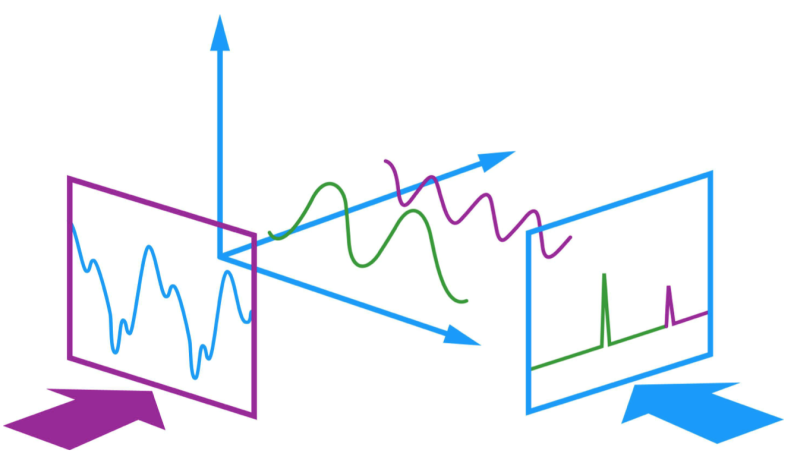
\includegraphics[width=0.7\textwidth]{Screenshot_20200217_122108.png}
\\
(Formule niet te kennen)1
\\
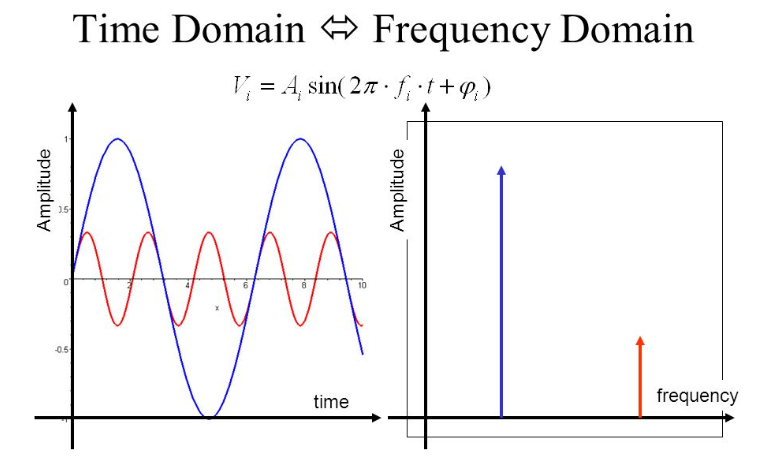
\includegraphics[width=0.7\textwidth]{Screenshot_20200217_122246.png}

\section{Digitale signalen}
Aan/uit


\subsection{Duty Cycle}
= Hoeveel procent van de tijd staat het signaal aan?

\subsection{Flanken (edge)}
\begin{itemize}
    \item Stijgende flank
    \item Dalende flank
    \item Belangrijk bij kloksignalen
\end{itemize}

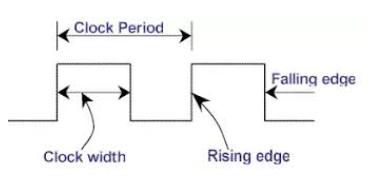
\includegraphics[width=0.5\textwidth]{Screenshot_20200217_123230.png}

\subsection{Weergave digitale signalen}
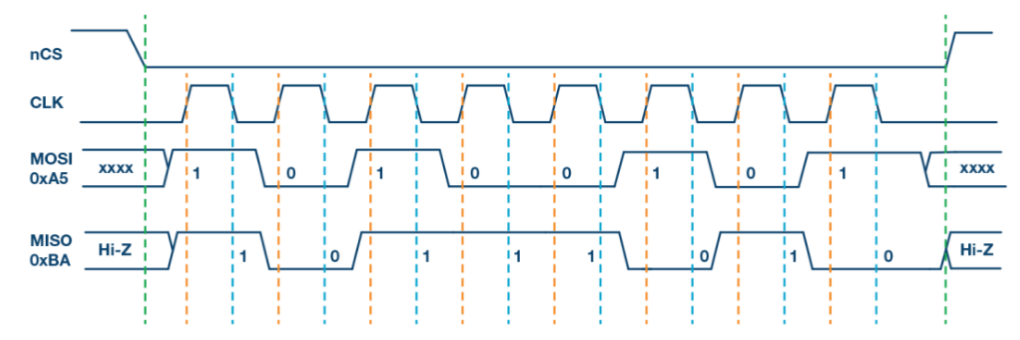
\includegraphics[width=1\textwidth]{Screenshot_20200217_125726.png}


\end{document}
